% !TEX root = ../main.tex
%
\chapter{Remaining Useful Lifetime Estimation}
\label{sec:rul_estimation}
\vspace*{-15mm}\hfill{\fontfamily{phv}\normalsize\emph{Vinay Kaundinya and Christopher Zinda}}

\cleanchapterquote{Better three hours too soon than a minute too late.}{William Shakespeare}{(Playwrite and poet)}

In this chapter, we present one of the most challenging Predictive Maintenance topics which is estimating the remaining useful lifetime (RUL) of a machine. We describe what RUL estimation is and why it is so important for manufacturers. In section~\ref{sec:rul_estimation:datasets} we provided a list of current datasets that can be used when testing a RUL approach. Section~\ref{sec:rul_estimation:approaches} will then give a deeper insight into six state-of-the-art approaches for predicting the RUL. The chapter closes with a summary of the most common metrics and loss functions that are used in combination with RUL estimation. In summary, this chapter will provide an insight into all important specifics to this PdM topic and the building blocks that are needed to implement RUL estimation.

\section{Motivation}
\vspace*{-12.5mm}\hfill{\fontfamily{phv}\normalsize\emph{Christopher Zinda}}
\label{sec:rul_estimation:motivation}

The 4th industrial revolution is presenting companies with enormous challenges. More and more processes are digitalized and the shopfloor is showing an increasing number of IoT devices. Most manufacturers equip their production lines with sensors that record a number of different properties. This enables them to collect large amounts of data that can be used for advanced Predictive Maintenance approaches.\\
One of the biggest cost factors in production is unscheduled downtime i.e. unexpected machine failure. Unexpected downtime is tied to immediate costs because the products can not be manufactured and will cause a delay for the customer. Also, replacement parts might not be in stock and even cause a greater delay until the production can continue. These unexpected events can occur when the statistical models that were created by experts do not reflect the real behavior. Due to the high complexity of these machines, there are also a lot of known and unknown variables that influence the Useful Lifetime of a machine. Using state-of-the-art approaches for RUL estimation, the risk of an unplanned downtime can be reduced by large amounts. The approaches try to learn the complex dependencies between the different sensors to obtain an approximate model of the machine. The main goal is to predict the time that a machine has left before a failure will occur. This can be achieved using any of the approaches that we describe in section~\ref{sec:rul_estimation:approaches}. With this information being known a priori the maintenance department can schedule a planned maintenance of the machine and ensure that replacement parts are already available. This way the costs can be drastically reduced. These types of machine learning approaches are slowly introduced in practice and there will be a lot of use cases in the future.

\subsection*{Challenges}
\label{sec:rul_estimation:motivation:challenges}

There are multiple challenges that arise when dealing with data driven approaches. Handling real time data from a factory implies a lot of unknown factors. We will describe some of the challenges that arise when trying to estimate RUL.

\subsubsection*{Health degradation trend}

For complex machines, it is very difficult to model their health degradation mathematically \cite{DBLP:journals/corr/abs-1709-01073}. There are many approaches that assume a certain degradation trend e.g. exponential degradation, but this might not relate to the true physical behavior of the machine. Often times there is no indication of the current health state, from which a degradation trend could be inferred. We will present some approaches in section~\ref{sec:rul_estimation:approaches} that do not rely on any degradation trend.

\subsubsection*{Noisy sensor readings}

The values that are recorded by the different sensors are often subject to noise. This can have various reasons. It depends on the quality of the equipment and sometimes also external factors like temperature and humidity in the factory. All these variables will add a small offset to the sensor reading such that it differs from the actual value. The approaches have to deal with this challenge because it is present in virtually any real-world application.

\subsubsection*{Partial unavailability}

The measurement of sensor information could be interrupted for a number of reasons. Production lines are typically very large and complex which makes it difficult to detail the different failure scenarios. However, it can always happen that the sensor gets damaged or that the connection is lost. This is true especially for wireless networks and it has to be accounted for.

\subsubsection*{Complex temporal dependencies between sensors}

Manufacturing machines are typically very complex and consist of a large number of components. Most of these components influence each other in a way that is very hard to model. A small change in hydraulic pressure could mean millimeters of deviation from normal operation, affecting a number of components down the line. The sensor might show different readings, but it is not possible to identify what caused them.

\section{Formal Definition}
\vspace*{-12.5mm}\hfill{\fontfamily{phv}\normalsize\emph{Christopher Zinda}}
\label{sec:rul_estimation:formal_definition}

A RUL estimation approach always uses a set of time series data (cf. \ref{sec:intro:time-series-definition}) as the input. When training the approach the training set $D_\text{train}$ contains the sensor information $x_i \in X$ of a machine for $N\in \mathbb{N}$ complete maintenance cycles. A maintenance cycle contains data for a machine from a running state until breakdown of the equipment. When using an unsupervised learning approach, the training set can be defined as:
\begin{equation} \label{eq:rul_train_set_unsupervised}
    D_\text{train} = \{x_i\}_{i=1}^N
\end{equation}
Supervised learning approaches use the following training set notation using a label $y_i \in Y$:
\begin{equation} \label{eq:rul_train_set_supervised}
    D_\text{train} = \{(x_i, y_i)\}_{i=1}^N
\end{equation}
Most approaches perform preprocessing on the input vectors $x_i$ using a different approach (e.g. health index estimation) and the actual RUL estimation is performed on an intermediate representation that varies from approach to approach.\\
The overall goal is then to predict an estimator function $h: X \rightarrow Y$ that is then used to get single scalar value $\hat{y}_i \in Y$ per Instance $x_i$ that is close to the actual RUL $y_i$ of the machine. The approach is evaluated on a test set $D_\text{test}$ with instances of time series data $x_i$ and a corresponding true RUL $y_i$ for every instance. The time series data $x_i$ however does not represent a full maintenance cycle, but ends some time before the breakdown of the equipment like in an online application scenario.
\begin{equation}
    D_\text{test} = \{(x_i, y_i)\}_{i=1}^M\quad, M \in \mathbb{N}
\end{equation}
Details on the evaluation metrics and used loss functions are described in \ref{sec:rul_estimation:evaluation_setup}.

\section{Available Datasets}
\vspace*{-12.5mm}\hfill{\fontfamily{phv}\normalsize\emph{Vinay Kaundinya}}
\label{sec:rul_estimation:datasets}

This section provides a description of two datasets, namely NASA C-MAPSS and PHM 2008 Data Challenge data set, that were used to test the state of the art approaches.
NASA C-MAPSS dataset consists of multivariate time series data which is simulated using a model based simulation called Commercial Modular Aero-Propulsion System Simulation by NASA. This dataset includes run-to-failure sensor measurements from degrading turbofan engines. As part of the dataset, 26 measurements were recorded.
Out of the 26 values, 1st value gives an unique ID for each Aircraft engine, 2nd value is the operational cycle number, 3rd to 5th value gives us 3 operational settings(1,2 and 3) and rest of the values are the values recorded from 21 different sensors. Table \ref{tab:rul_table1} gives us as an idea of the Dataset schema followed in the C-MAPSS dataset.

\begin{table}[ht]
    \begin{tabularx}{\textwidth}{ X | X | X }
        \hline
        \textbf{DataFields} & \textbf{Types} & \textbf{Descriptions} \\ \hline
        ID                  & Integer        & 2                     \\ %\hline
        Cycle               & Integer        & 5                     \\ %\hline
        Setting 1           & Double         & 5                     \\ %\hline
        Setting 2           & Double         & 5                     \\ %\hline
        Setting 3           & Double         & 5                     \\ %\hline
        S1                  & Double         & Sensor Measurement 1  \\ %\hline
        S2                  & Double         & Sensor Measurement 2  \\ %\hline
        ..                  & ..             & ..                    \\ %\hline
        S21                 & Double         & Sensor Measurement 21 \\ \hline
    \end{tabularx}
    \caption{Dataset Schema}
    \label{tab:rul_table1}
\end{table}

\begin{table}[ht]
    \begin{tabular}{ p{2.2cm}  p{9cm}  p{1.3cm} }
        \hline
        \textbf{Symbol} & \textbf{Description}                                 & \textbf{Unit} \\
        \hline
        T2              & Total temperature at fan inlet                       & $^{\circ}$R   \\
        T24             & Total temperature at Low Pressure Compressor outlet  & $^{\circ}$R   \\
        T30             & Total temperature at High Pressure Compressor outlet & $^{\circ}$R   \\
        T50             & Total temperature at Low Pressure Turbine outlet     & $^{\circ}$R   \\
        P2              & Pressure at fan inlet                                & psia          \\
        P15             & Total pressure in bypass-duct                        & psia          \\
        P30             & Total pressure at HPC outlet                         & psia          \\
        Nf              & Physical fan speed                                   & rpm           \\
        Nc              & Physical core speed                                  & rpm           \\
        epr             & Engine pressure ratio (P50/P2)                       & --            \\
        Ps30            & Static pressure at HPC                               & psia          \\
        phi             & Ratio of fuel flow to Ps30                           & pps/psi       \\
        NRf             & Corrected fan speed                                  & rpm           \\
        NRc             & Corrected core speed                                 & rpm           \\
        BPR             & Bypass Ratio                                         & --            \\
        farB            & Burner fuel-air ratio                                & --            \\
        htBleed         & Bleed Enthalpy                                       & --            \\
        $Nf_{dmd}$      & Demanded fan speed                                   & rpm           \\
        $PCNFR_{dmd}$   & Demanded corrected fan speed                         & rpm           \\
        W31             & High Pressure Turbine coolant bleed                  & lbm/s         \\
        W32             & Low Pressure Turbine coolant bleed                   & lbm/s         \\
        \hline
    \end{tabular}
    \caption{C-MAPSS Dataset Sensor Descriptions}
    \label{tab:rul_table2}
\end{table}

Furthermore, 21 different sensor values recorded in the C-MAPSS dataset with their descriptions and unit of measure are as listed in table \ref{tab:rul_table2}.

Like most datasets, C-MAPSS dataset is also divided into Training data, Testing data and Ground truth data. C-MAPSS dataset consists of time series information of all the turbofan engine sensors at 100 different instances. These recordings are stored under train\_FD001.txt and act as the training data, as it contains data from the beginning to end of its usage. Testing data which is contained in test\_FD001.txt, we consider the time series recordings for another 100 instances where the time series has information until some prior time to its failure. This will enable us to estimate their RUL using our approaches and then compare to its ground truth data which is stored in RUL\_FD001.txt.
PHM 2008 Data challenge dataset is also simulated data produced using the same model based program C-MAPSS, by NASA. This dataset is structured exactly the same way as described above for the C-MAPSS dataset. However the only physical difference is, while for each of the C-MAPSS dataset the actual RUL values are made available, the actual RUL values in PHM Data Challenge dataset is not available.

\section{State-of-the-art Approaches}
\vspace*{-3mm}\hfill{\fontfamily{phv}\normalsize\emph{Vinay Kaundinya and Christopher Zinda}}
\label{sec:rul_estimation:approaches}

In this section we describe six state-of-the-art approaches that can be used to estimate the remaining useful lifetime.

\subsection{Embed-RUL using RNN}
\vspace*{-12.5mm}\hfill{\fontfamily{phv}\normalsize\emph{Christopher Zinda}}
\label{sec:rul_estimation:approaches:embed_rul}

The idea behind Embed-RUL is to use a series of embeddings to estimate a health index which is then used to generate a prediction of the remaining useful lifetime. We will describe and summarize the findings of \cite{DBLP:journals/corr/abs-1709-01073} in this chapter to provide an understanding of this approach. What is special in contrast to other approaches is that the input for the HI Estimation is generated from the time series data by a Recurrent Neural Network Encoder (see Figure~\ref{fig:embed_rul}).
\begin{figure}[ht]
    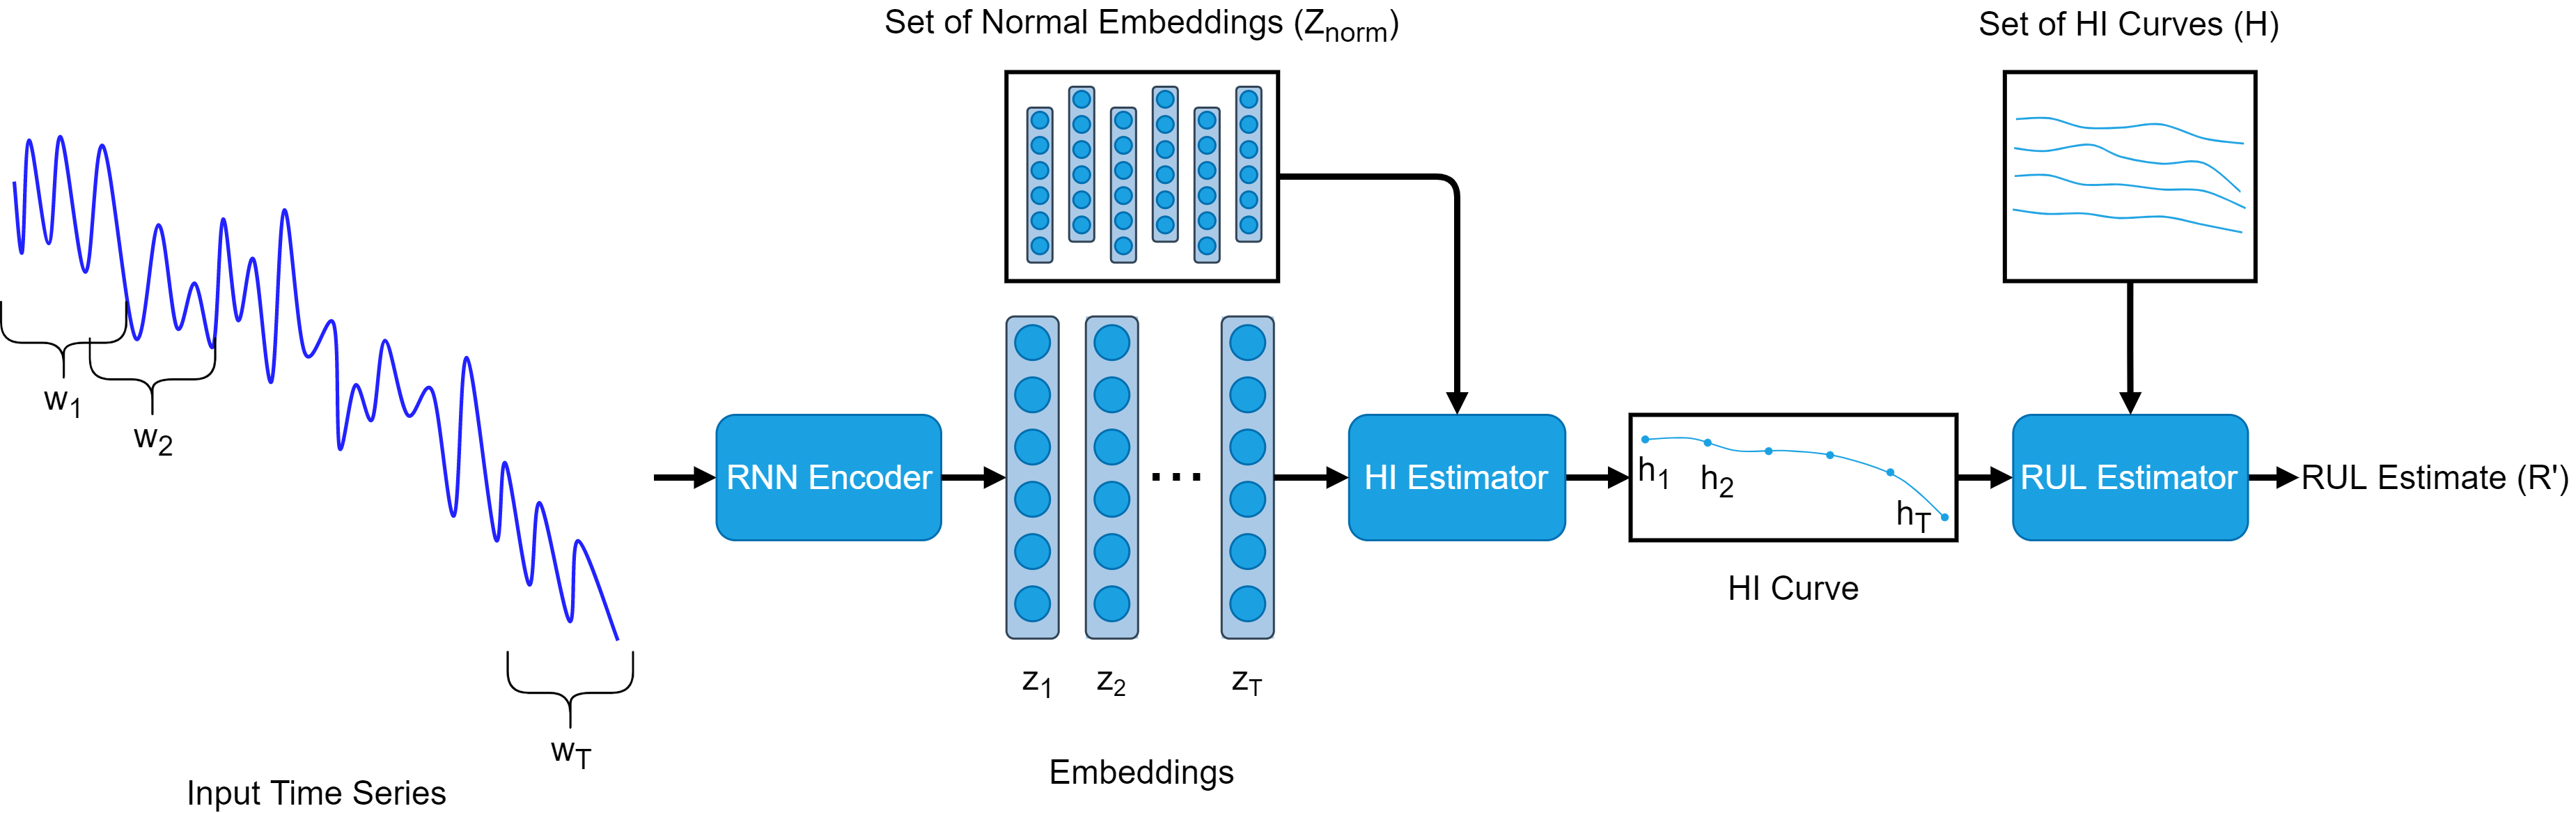
\includegraphics[width=\textwidth]{gfx/rul_embed_rul_pipeline.drawio}
    \caption{Embed-RUL pipeline \cite{DBLP:journals/corr/abs-1709-01073}.}
    \label{fig:embed_rul}
\end{figure}

The pipeline has three different stages that take the raw time series data, transform it into different intermediate representations and generate a RUL estimation in the end. These three stages are described in the following paragraphs.

\subsubsection*{RNN Encoder Decoder Learning}
\label{sec:rul_estimation:approaches:embed_rul:rnn_encoder_decoder_learning}

The time series data is first divided into windows of length $w\in \mathbb{N}$ with maximum overlap (i.e. to create the next window just add the next more recent value and remove the oldest value). The goal of this first step is then to create an embedding $z_i^{(t)} \in \mathbb{R}^c$ (where $c$ is the total number of recurrent units in the RNN Encoder) that serves as a short representation of the time series data in this window.\\
The RNN Encoder Decoder is then trained to obtain functions $f_\text{enc}$ and $f_\text{dec}$ like the following:
\begin{equation}
    \begin{aligned}
        \text{Generate embedding: } z_i^{(t)} = f_\text{enc}(x_i^{(t - w + 1, t)}) \\
        \text{Reconstruct time series: } \widetilde{x}_i^{(t - w + 1, t)} = f_\text{dec}(z_i^{(t)})
    \end{aligned}
\end{equation}
The reconstruction error for training the RNN Encoder Decoder is then given by:
\begin{equation}
    e_i^{(t)} = \sum_{j=(t-w+1)}^t ||x_i^{(j)}-\widetilde{x}_i^{(j)}||^2
\end{equation}
The RNN-ED is then trained to minimize the loss function that sums up the reconstruction error for all windows of time series data and all training set instances where $T\in \mathbb{N}$ denotes the last time step for the training instance:
\begin{equation}
    \mathcal{L} = \sum_{i=1}^N \sum_{t=w}^T e_i^{(t)}
\end{equation}
This provides us with a very robust RNN Encoder that generates a condensed representation of the time series data for use in the next stage.

\subsubsection*{HI Estimator}
\label{sec:rul_estimation:approaches:embed_rul:hi_estimator}

The generated embeddings $z_i^{(w)}, \ldots, z_i^{(T)}$ are then used to perform a health index estimation. The individual embeddings are compared to the embeddings of a normal operation which are maintained in a set $Z_{norm}$. The health index is then achieved as follows:
\begin{equation}
    h_i^{(t)} = min(||z_i^{(t)} - z||) \quad \forall z \in Z_{norm}
\end{equation}
In this notation a low value means a good health because it is close to the normal operation. However this result can be inverted and normalized to obtain a classical health index estimation where 0 means bad and 1 means good health. A health index curve is then denoted like follows:
\begin{equation}
    h_i = \{h_i^{(w)}, h_i^{(w+1)}, \ldots, h_i^{(T)}\}
\end{equation}

\subsubsection*{RUL Estimator}
\label{sec:rul_estimation:approaches:embed_rul:rul_estimator}

The RUL estimation is generated by comparing the HI curve $h_{i^*}$ for a test instance $i^*$ with the HI curves in the set $H$ that contains normal operation values (see Figure~\ref{fig:embed_rul}). The similarity is expressed by the following formula where $T^{(i^*)}$ denotes the last recorded time step for the test instance:
\begin{equation}
    s(i^*, i, t_D) = \exp \left(-\frac{1}{T^{(i^*)}}\sum_{k=w}^{T^{(i^*)}}\left(h_{i^*}^{(k)}-h_i^{(k+t_D)}\right)^2/\lambda\right)
\end{equation}
$\lambda > 0,\ \  t_D\in \{1,2,\ldots,\tau\},\ \  t_D+T^{(i^*)}\leq T^{(i)}$ where $\tau$ denotes the maximum allowed time lag $t_D$ and $\lambda$ scales the term to control how close two health curves have to be. The final RUL is then given by a weighted average using all combinations of $i$ and $t_D$ that satisfy the constraints $s(i^*, i, t_D)\geq\alpha\cdot s_{max}$, where $s_{max}=\max_{0\leq i\leq N, t_D\in \{1,\ldots \tau\}}\{s(i^*, i, t_D)\},\ \  0\leq \alpha\leq 1$. This results in the following formula for the RUL estimate:
\begin{equation}
    R_{i^*} = \frac{\sum s(i^*, i, t_D)\cdot (T^{(i)}-T^{(i^*)}-t_D)}{\sum s(i^*, i, t_D)}
\end{equation}

\subsection{Direct RUL using SVR}
\vspace*{-12.5mm}\hfill{\fontfamily{phv}\normalsize\emph{Vinay Kaundinya}}
\label{sec:rul_estimation:approaches:direct_rul}

%Approaches for RUL estimation have been broadly classified into 3, Model based, Data driven and Hybrid. Model based approaches require specific domain knowledge in building physical models and hence its applicability decreases. Data driven models use statistical learning methods in approximating the system's behavior, based on regularly collected past data. Use of such approaches can offer a tradeoff between precision and applicability. Hybrid approaches are a combination of specific domain knowledge and collected system data.

Most RUL estimation approaches proposed in the literature, have been two stepped. The first step deals with the estimation of health state of the machine and followed by a simple calculation of RUL. However the method proposed in \cite{DBLP:journals/tie/KhelifCMLFZ17} , "\textit{Direct RUL using Support Vector Regression}" is able to estimate RUL without estimating the health states, but directly using the collected sensor data.
\begin{figure}[ht]
    \centering
    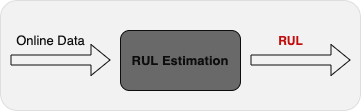
\includegraphics[width=0.5\textwidth]{gfx/rul_direct_rul}
    \caption{Direct RUL estimation \cite{DBLP:journals/tie/KhelifCMLFZ17}}
    \label{fig:direct_rul}
\end{figure}

For Direct RUL approach to take the denoised sensory data as input and output the RUL value, the approach needs to extract the required senor features that can help in associating it to the RUL value. A wrapper method is then used to optimize the number of sensors observed, only the relevant sensor data is taken and the other sensors' data is ignored. This method can be realized in the following 4 steps:

\textit{1: Data sensor selection}: Here the wrapper method is used to select the most relevant sensors.\\
We understand that with any dataset, there exists a good percentage of irrelevant or redundant information and training a model with everything can lead to inaccurate results. Hence it is necessary to filter only relevant information in developing a robust model. Broadly feature selection approaches can be classified into filters, wrappers and embedded methods.
Here we choose wrapper methods, where selection criterion is dependent on the performance of the mining algorithm. This is known to be a time consuming process and hence it is done as a offline process with data only for 5 sensors.

\textit{2: Training set construction}: Here we construct the training set mapping features and their RUL values.\\
First step is to decompose the time series $T_{i}$ into non overlapping windows of size \textit{L}. One of the windows in the time series $T_{i}$, \textit{k}th window can be shown to contain $t^{i}_{(k-1),L+1},,,t^{i}_{kL}$ \cite{DBLP:journals/tie/KhelifCMLFZ17}.
We extract two parameters per dimension, average value \textit{a} and regression trend coefficient \textit{s} for each window. When \textit{d} is the dimensions of the time series $T_{i}$, a feature vector of size \textit{2 X d} is computed. Remaining useful lifetime value can be calculated as follows $$l(T_i) - kL$$
Each vector is then associated with a Remaining useful lifetime value to give us the training set $$D_\text{train} = \{x_i, y_i\}_{i=1}^{N}$$ where \textit{$x_i$}$\in R^{2d}$ and \textit{$y_i$} is the RUL value of the window from its last instant. Here the RUL value is also added to priorly defined $D_\text{train}$.
\begin{figure}[ht]
    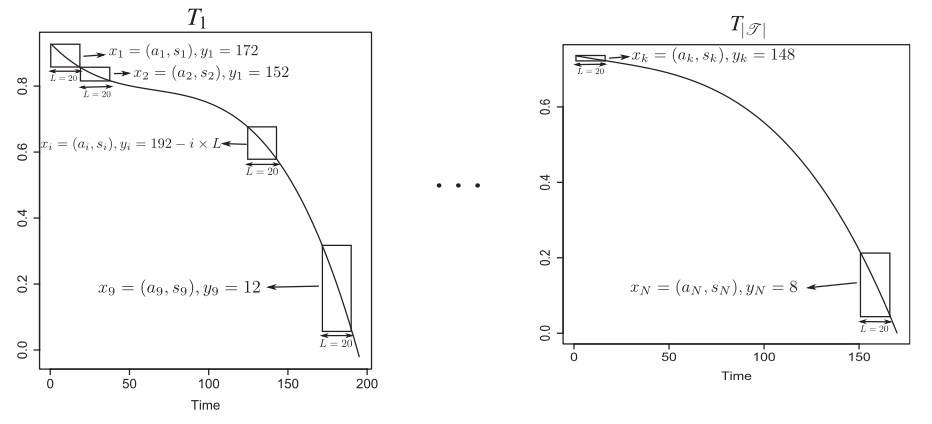
\includegraphics[width=\textwidth]{gfx/rul_trendfeats}
    \caption{An example of windowing technique, $L = 20$, $l(T_{1}) = 192$. \cite{DBLP:journals/tie/KhelifCMLFZ17}}
    \label{fig:trendfeats_rul}
\end{figure}

\textit{3: Learning an SVR model}: We train the SVR model with our training data with relationships between predictor and target variables.\\
In this step, we use the predictor variables $x$ to predict the target variable $y$ using regression technique. We use SVR to model the relationships between predictor and target variables.
$\nu$ SVR and $\epsilon$ SVR are the two types of SVR. Looking at minimizing the error, $\epsilon$ SVR is chosen where parameter $\epsilon$ controls the amount of error allowed in the model. $\epsilon$ SVR looks to work on minimizing $\mid \mid \omega \mid \mid^{2}$ such that,
$$
    \begin{cases}
        y_{i} - \langle \omega,x_{i} \rangle - b \leq \epsilon \\
        \langle \omega,x_{i} \rangle + b - y_{i} \leq \epsilon
    \end{cases}
$$
where $\big \langle .,. \big \rangle$ is the dot product and $\omega$ is the separating plane in a high dimensional space ($\Re^{2d}$). The above conditions might not always satisfy $\epsilon$ margin condition, hence new slack variables $\zeta_{i}$ and $\zeta_{i}^{*}$ are introduced. As in SVM, the kernel trick is used where the input data are mapped into a feature space. The $\epsilon$ SVR is then used to model the non-linear relationships between $x$ and $y$. This is nothing but the model $m$ that can help us find the RUL of components.

\textit{4: Prediction of RUL}: Here we predict the RUL values for the test data.\\
SVR trained as described above is now used to predict the RUL values. Here the model uses the time series $U = \{u_{i}\}_{i = 1}^{l(U)}$. This model aims to predict the time difference between $l(U)$ and the time at which the failure occurs.
In this step we split the time series into windows of size L. A new window($n_{U}$) is obtained by shifting the previous one by one time unit, i.e $n_{U} = l(U) - L + 1$. From each of these $U$ windows a $2d$ feature vector is obtained by extracting the trend features as explained in steps above.

If $x_{k}$ is the feature vector of the $k$th window in the time series, $x_{k}$ is passed to the SVR model $m$ which predicts $y_{k}$, the time at which the failure is supposed to occur. The time is calculated using $\hat{f}_{k} = L + k - 1 + y_{k}$. This will lead to $n_{U}$ such predictions and an average or weighted average of these values gives us the final RUL value of the time series.

\subsection{Random Forests}
\vspace*{-12.5mm}\hfill{\fontfamily{phv}\normalsize\emph{Christopher Zinda}}
\label{sec:rul_estimation:approaches:random_forests}

Random Forests were successfully applied to predict the remaining time until a product becomes obsolete \cite{GSCH:jennings2016forecasting}. It has also been shown that the RUL prediction using Random Forests achieves very low root mean squared error values when compared to other conventional machine learning algorithms \cite{GSCH:mathew2017prediction}. This is why we included the approach in this survey and we will describe it in greater detail in the following section. The explanation of Random Forests is mainly based on the paper by Cutler et al. \cite{GSCH:cutler2012random}.

The approach uses a number of different decision trees and averages their predictions to get a final RUL prediction. From the two available tree types (classification and regression) we are using regression trees because they fit the PdM problem domain. The main issue of decision trees however is that they can be inaccurate and prone to overfitting. This is why multiple regression trees are used and their predictions are averaged.\\
regression trees are binary trees that divide the instances of sensor data into multiple partitions. In Figure~\ref{fig:decision_tree_rul} you can see an example with fictional values. Three sensors were recorded (temp, energy\_use, oil\_pressure) and based on their specific values the decision tree makes a prediction of the RUL. The RUL is denoted in days at the leaf nodes.
\begin{figure}[ht]
    \centering
    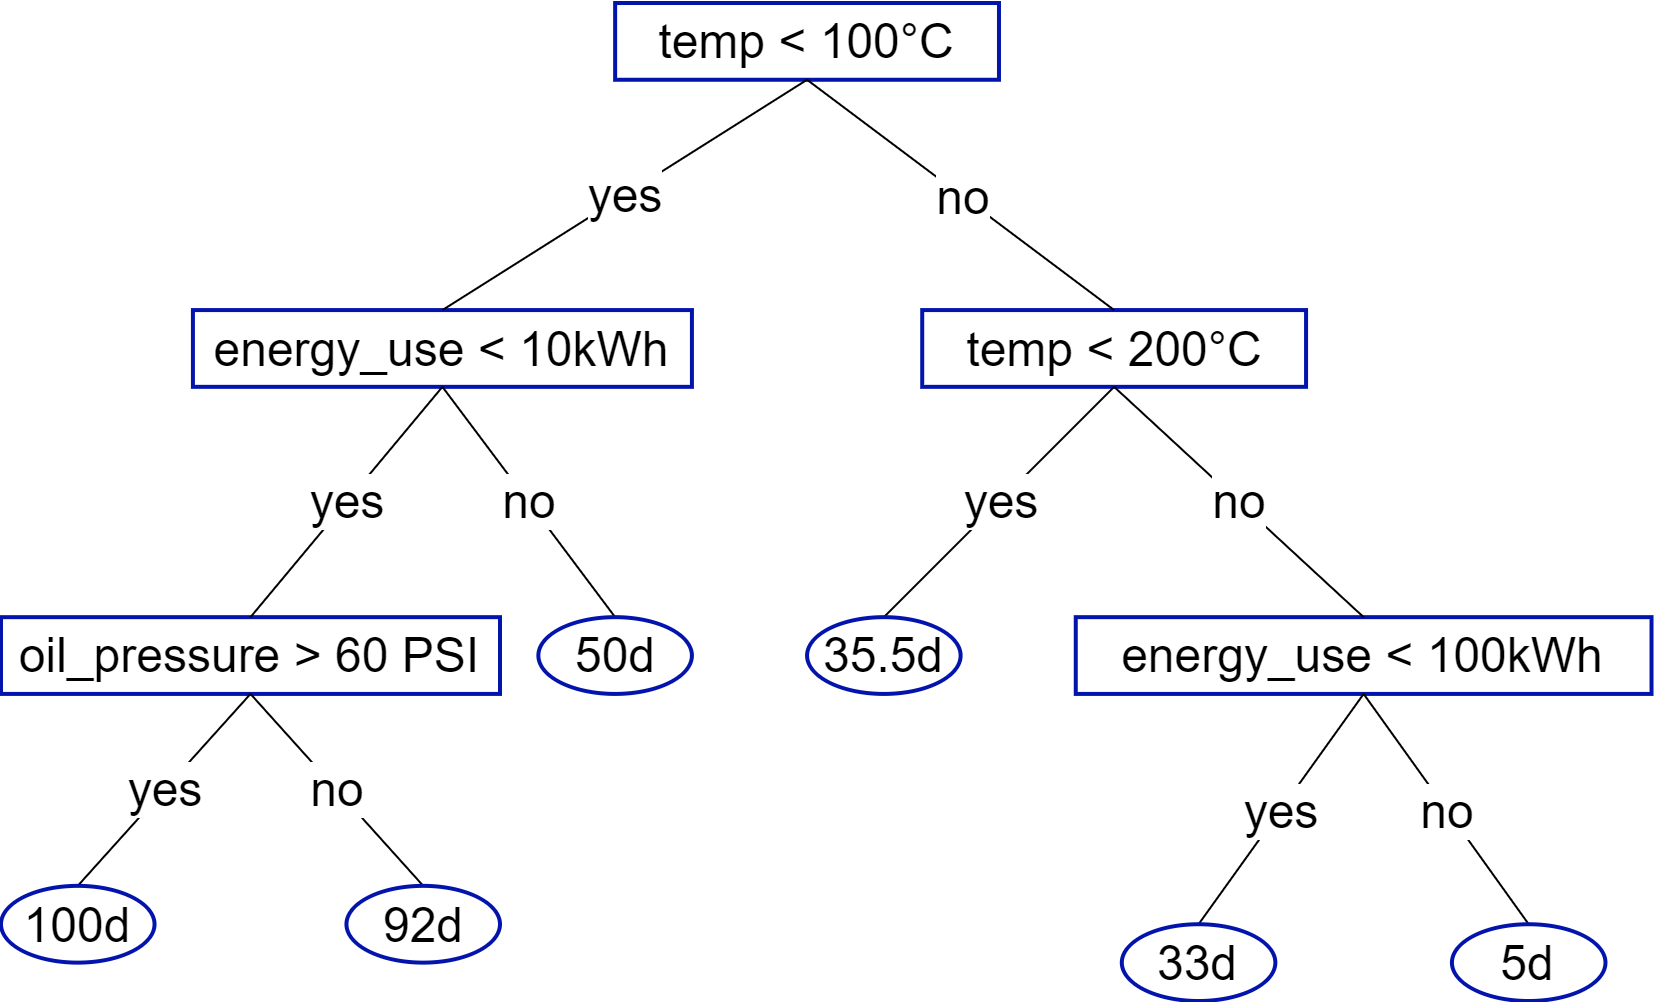
\includegraphics[width=0.8\textwidth]{gfx/rul_decision_tree.drawio}
    \caption{Example of a decision tree for RUL estimation with fictional values.}
    \label{fig:decision_tree_rul}
\end{figure}

A single regression tree is trained by using Binary Recursive Partitioning (BRP). The training set for this algorithm is constructed as follows.
\begin{equation} \label{eq:rul_random_forests_training_set}
    D_\text{train} = \{(x_1, y_1), \ldots, (x_P, y_P)\} \text{ with } x_i = (v_{i,1}, \ldots, v_{i,S})^T
\end{equation}
where $P$ is the total count of all time steps for the $N$ maintenance cycles (i.e. the overall count of sensor readings) and $y_i$ denotes the RUL at the point in time when the sensor values $x_i$ were recorded.\\
The algorithm starts with all training set instances $(x_i, y_i)$ in the root node and searches for the best split among all $S$ sensors. To find the best split, all possible values $v_{i, j}$ for a fixed sensor $j$ are sorted and a split between every distinct pair of values is considered. The threshold of a split is denoted by $c\in \mathbb{R}$ which means that all instances $x_i$ where $v_{i,j} < c$ will be propagated to the left subtree. The remaining instances will be propagated to the right tree. For all values of $c$ and all sensors $j\in [S]$ the score of the split $Q_\text{split}$ is evaluated.
\begin{equation}
    Q_\text{split} = n_LQ_L+n_RQ_R
\end{equation}
where $n_L$ and $n_R$ denote the number of instances that are assigned to the left and right subtree. $Q_L$ and $Q_R$ are evaluated by computing $\frac{1}{n}\sum_{i=1}^n(y_i-\overline{y})^2$ for the left and right subtree. $\overline{y}$ is the average of all labels $y_i$ for the respective subtree which means that $Q_L$ and $Q_R$ can be seen as a measure of similarity. Finally, the split is chosen that minimizes $Q_\text{split}$ and the algorithm works on the two resulting subtrees recursively. The recursion is stopped once a stopping criterion is met and there is no point in further partitioning the data. The stopping criterion could be a smallest number of instances in a leaf node or a maximum number of leaf nodes.\\
Once the training is finished we can use the regression tree to get a RUL prediction for a test instance $x_{i^*}$ by propagating it through the tree based on the recorded sensor values and split thresholds. When a leaf node $k$ is reached, the RUL estimate is computed by taking the average over all labels $y_{k_i}$ of the training data associated with that node.
\begin{equation}
    \hat{h}(x_{i^*}) = \frac{1}{n}\sum_{i=1}^n y_{k_i}
\end{equation}
As described before it is not sufficient to use only a single decision tree. Instead we want to use multiple trees that are trained differently and average over their predictions to get a robust RUL prediction.\\
Let $J$ denote the number of trees that will be trained by the Random Forests algorithm. First the algorithm will obtain a bootstrap sample $D_j$ of size $P$ from the original training set. A bootstrap sample is generated by randomly picking a number of training set instances. After one iteration the instances are placed back in the training set and new instances are randomly selected which opens the possibility for duplicates in the bootstrapped sample set. After the bootstrapping is finished, a regression tree will be trained on that sample, but with a modification to the Binary Recursive Partition algorithm. Instead of searching for a best split on all $S$ sensors, the BRP algorithm will only search on a random selection of $m < S$ sensors.\\
The bootstrapping of the training set and the random selection of sensors ensure a high randomization for the different decision trees. Once all $J$ trees have been trained that way, we can get a robust RUL prediction by averaging over all trees:
\begin{equation}
    R_{i^*} = \frac{1}{J}\sum_{j=1}^J \hat{h}_j(x_{i^*})
\end{equation}

After it was described how the Random Forests algorithm works, we will take a look at the parameters of the approach. There are three parameters which are subject to optimization: $m$ (number of randomly selected sensors), $J$ (number of trees) and the stopping criterion. Usually the default selection for $m$ is $P/3$ and there is no need to do much fine-tuning because overfitting effects due to $m$ are very low. The selection of $J$ however worsens the generalization error if it is chosen too low. $J$ should be selected rather high to get to the point where the generalization error converges. This can be ensured by plotting the Out-Of-Bag (OOB) error for some values of $J$. The OOB error can be computed for the training set instances that were not taken during bootstrap sampling. Lastly, the original work on Random Forests suggests to use a stopping criterion that allows for very large decision trees \cite{GSCH:cutler2012random}. It has to be considered that a large tree size can cause overfitting and the stopping criterion has to be adapted to prevent this.

Random forests have a number of advantages that make them appealing. As shown above, Random Forests only have a few parameters that need to be tuned. Also they have a built-in estimate of the generalization error by computing the OOB error. Lastly, they can be implemented in parallel which makes the training relatively fast. To conclude, Random Forests provide a powerful tool for predicting the RUL of a machine.

\subsection{CNN based Regressor}
\vspace*{-12.5mm}\hfill{\fontfamily{phv}\normalsize\emph{Vinay Kaundinya}}
\label{sec:rul_estimation:approaches:cnn_rul}

Estimation of remaining useful lifetime of a component or a subsystem becomes crucial in varied application areas like manufacturing, aerospace etc. Existing algorithms in predicting RUL of a component are all based on multivariate analysis or damage progression analysis. To accurately predict RUL becomes challenging if there is no good representation of features. In the paper \cite{DBLP:conf/dasfaa/BabuZL16}, the authors Giduthuri Sateesh Babu, Peilin Zhao, and Xiaoli Li  proposed an approach that estimates RUL as a multivariate time series regression task based on Convolutional Neural Network(CNN), adapted from deep learning techniques for image classification.

As part of the approach, a sliding window strategy is adopted to segment the multivariate time series data into short segments of signals. These signals($r$) along with their attributes($D$) then form a 2 dimensional  matrix ($r \times D$), which forms as an instance of input to CNN. In case of single operating condition, the raw signals($d$) becomes the input. However in case of multiple operating conditions dataset, raw sensor signals and the features attributed to operating conditions are included. Here, we use 2 pairs of convolution layers and pooling layers and finally connected to a multi layered perceptron for RUL estimation. In CNN, $r$ (windowing rate or sampling rate) is chosen to be 15 and step size of 1. First we feed the segmented multivariate time series($D \times 15$) as input through 2 layers of convolution and pooling layers. Then all the feature maps are concatenated at the end of the last pooling layer into a vector input for MLP for RUL estimation.
\begin{figure}[ht]
    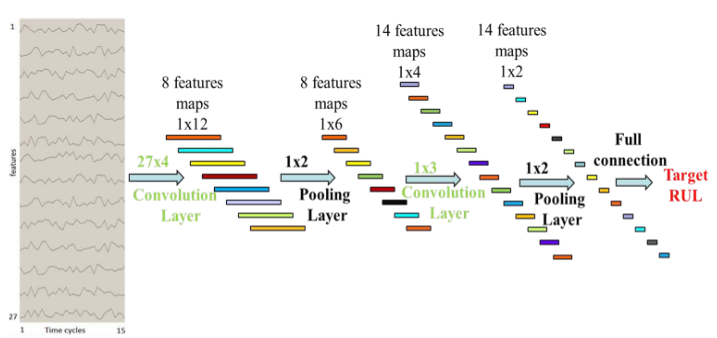
\includegraphics[width=\textwidth]{gfx/rul_cnn_architecture}
    \caption{CNN architecture proposed to estimate RUL. It includes 2 pairs of convolution and pooling layers and a fully connected MLP layer. \cite{DBLP:conf/dasfaa/BabuZL16}}
    \label{fig:cnn_archi_rul}
\end{figure}

In convolution layers, the input from the previous layer is convolved using a kernel that is learned during training. Then the activation function computes the next layer feature maps,
\begin{equation}
    x_{j}^{l} = sig(z_{j}^{l}),    z_{j}^{l} = \sum_{i}x_{i}^{l-1} * k_{ij}^{l} + b^{l}_{j}
\end{equation}
Here, * is the convolution operator, $x_{i}^{l-1}$ and $x_{j}^{l}$ are the input and output of the convolutional layer and $sig()$ denotes the sigmoid function. We apply first convolution filter of size $D \times 4$ in the first layer and of size $1 \times 3$ in the second layer.

In pooling layers, features output from the convolution layer is then segmented or sub-sampled into set of non overlapping data, to increase the invariance of features to distortions on the inputs. Here we use the average pooling, to get the average value of the sub-samples as its output.
\begin{equation}
    x_{j}^{l+1} = down(x_{j}^{l})
\end{equation}
where, $x_{j}^{l}$ is the input to the pooling layer and $x_{j}^{l+1}$ is the output. $down()$ acts as the sub-sampling function for average pooling. The size of both the pooling layers is $1 \times 2$.

In training the proposed CNN approach, we use the squared error loss function and the procedure consists of phases of forward propagation, backward propagation and the application of gradients. The loss function is defined as follows:
\begin{equation}
    E = 1/2(y(t) - y^{*}(t))^2
\end{equation}
where $y(t)$ is the target RUL and $y^{*}(t)$ is the predicted RUL value.

\textbf{Forward propagation} deals with computing output feature maps of each layer and also the output of CNN model as whole. The outputs of the convolution and pooling layers are computed using equations 5.11 and 5.12 respectively. These outputs are then fed into a single fully connected layer.
Once after an iteration of forward propagation, the error value after squared error loss function is available. \textbf{Backward propagation} is initiated and deals with error value and propagates from the last layer to first. As the errors propagate from last layer to first, derivatives are calculated using following functions,

$up()$: This function has an inverse operation of the $down$ function as defined above. \\
$reverse()$: This reverses the function of feature extractors. \\
$pad()$: Adds zeroes as padding, as described in the paper \cite{DBLP:conf/dasfaa/BabuZL16}.

Once we get the values of parameter derivatives we apply them to update the parameters. If $E(w)$ is the cost function that we try to minimize, then \textbf{Gradient} descent suggest to modify the values in the direction of its steepest descent, such that
\begin{equation}
    w^{l}_{ij} = w^{l}_{ij} - \eta \frac{\delta{E}}{\delta{w^{l}_{ij}} }
\end{equation}
Here $w_{ij}$ is the weight to be modified and $\eta$ is the learning rate that will determine how much modification the weight will have. Larger the $\eta$, greater the modification of $\omega_{ij}$.

\subsection{Multiple Classifier Approach}
\vspace*{-12.5mm}\hfill{\fontfamily{phv}\normalsize\emph{Christopher Zinda}}
\label{sec:rul_estimation:approaches:multiple_classifier_approach}

The Multiple Classifier Approach as described in the paper by Susto et al. trains multiple classification modules with different prediction horizons to gain information about the best time to do maintenance with minimal costs \cite{DBLP:journals/tii/SustoSPMB15}. The following chapter therefore describes the findings of that paper to provide you with an insight in this different approach and shows how it can be applied to the prediction of RUL.

The training set for the approach is defined like in equation~\ref{eq:rul_random_forests_training_set} where $P$ is the total count of all time steps for the $N$ maintenance cycles (i.e. the overall count of sensor readings), but $y_i$ has a different meaning. If there was a breakdown of the machine at time step $i\in[P]$, then the label is \textit{faulty} (F). Otherwise it is \textit{not faulty} (NF):
\begin{equation}
    y_i = Y(i) = \begin{cases}
        \text{F,}  & \text{if iteration }i\text{ is faulty}     \\
        \text{NF,} & \text{if iteration }i\text{ is not faulty}
    \end{cases}
\end{equation}
However, this would cause the dataset to be very unbalanced and skewed. With the current definition there are $N$ faulty instances and $P-N$ instances that are not faulty. Typically $P\gg N$ which results in an unbalanced training set and will cause poor prediction accuracy and generalization.\\
To mitigate this issue, the Multiple Classifier Approach trains several classifiers on training sets with varying failure horizon $m\in\mathbb{N}$. The failure horizon defines the number of instances at the end of a maintenance cycle that will be marked as faulty:
\begin{equation}
    y_i^{(t)} = \begin{cases}
        \text{F,}  & \text{if }t > n_i - m_j \\
        \text{NF,} & \text{otherwise}
    \end{cases}
\end{equation}
where $t$ is the time step in the $i$th maintenance cycle which has length $n_i$ and $m_j$ denotes the failure horizon for the $j$th classifier.\\
The type of classifier can be chosen independently. In the cited paper they are using k-NN which is a simple classifier and SVM which yields slightly better results.

The approach that is suggested in the paper by Susto et al. uses a training and an additional validation set to perform crossvalidation \cite{DBLP:journals/tii/SustoSPMB15}. They are obtained by randomly splitting the maintenance cycles using a factor $0 < q < 1$ such that $N_\text{train} = \lfloor Nq\rfloor$ and $N_{val} = \lceil N(1-q)\rceil$.\\
To train a single classifier, the algorithm first executes a number of $Q$ simulations to tune the hyperparameters. In every simulation random training and test sets are obtained using the factor $q$. The misclassification rate (MCR) is then evaluated for different hyperparameters. Based on these results, the hyperparameters are chosen that had the lowest average MCR over all simulations. This whole process is repeated for each of the $J$ classifiers using their specific failure horizon $m_j$. The failure horizon for the $j$th classifier should be set to $m_j = j$. This results in $J$ trained and fine-tuned classifiers that can be used to predict the RUL.

Because we trained the classifiers in a way that the $j$th one learns to predict a failure when there are less than or equal to $j$ time steps left (failure horizon $m_j = j$), we can obtain the actual RUL prediction by finding the lowest index $j^*$ such that all classifiers with index $j \geq j^*$ predict F.
\begin{equation}
    R_{i^*} = \min j^* \::\: \hat{h}_j(x_{i^*}) = \text{F},\quad \forall j \geq j^*
\end{equation}
where $\hat{h}_j$ is the output of the $j$th classifier.

\subsection{Long Short-Term Memory}
\vspace*{-12.5mm}\hfill{\fontfamily{phv}\normalsize\emph{Vinay Kaundinya}}
\label{sec:rul_estimation:approaches:lstm_rul}

From the different approaches we have described above, we can say that regression based and neural network based models extract features from the segmented windows of the time series data. However, these techniques face issues in accurately modelling long term dependencies and when modelling sequence information. We now describe a Long Short Term Memory (LSTM) approach for RUL estimation as proposed in the paper \cite{DBLP:conf/icphm/ZhengRFG17} by the authors Shuai Zheng, Kosta Ristovski, Ahmed K Farahat, and Chetan Gupta. This approach looks at making full use of the sensor data in extracting the required feature information, leveraging multiple layers of LSTM cells.

According to definition $\mid s\mid$ is the number of sensors, here a $\mid s\mid$-dimensional time series data is passed as input to the $LSTM$ model and $y$ as estimated RUL value is the output. The proposed model is consists of multiple layers of LSTM cells followed by a feed forward neural networks(NN). Each LSTM layer is then made up of sequence of LSTM cells. A typical LSTM model looks as shown in figure \ref{fig:lstm_rul}.
\begin{figure}[ht]
    \centering
    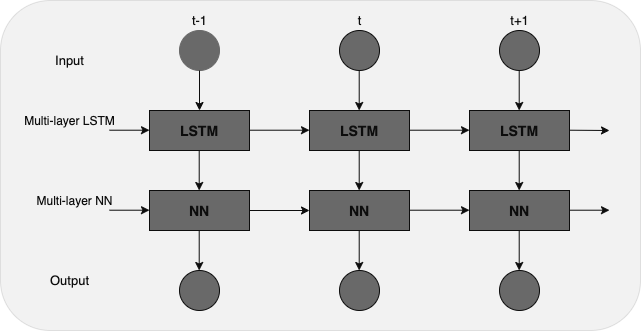
\includegraphics[width=0.7\textwidth]{gfx/rul_lstm1}
    \caption{LSTM Model. \cite{DBLP:conf/icphm/ZhengRFG17} }
    \label{fig:lstm_rul}
\end{figure}

Output of an LSTM cell is a value $h^t$ and also its state $c^t$, both of which are vectors of the same size at time instant $t$. Size of these vectors are defined by the number of nodes($m$) a cell contains. As each layer is a sequence of such cells, the output($h^{t-1}$) and state($c^{t-1}$) of a LSTM cell at time $t-1$ becomes the input for the next LSTM cell at time $t$. Each cell consists of 3 gates: input gate($i^t$), output gate($o^t$) and forget gate($f^t$). Input gate controls the information that will be passed on from the previous cell $h^t$ and the time series input data $x^t$. Output gate controls what will be passed on to the next cell. Forget gate is responsible for controlling information what a cell will retain as memory.

In the proposed approach, different variable weights and biases that will be computed during the training process in each cell are denoted by $W$, $U$ and $b$. $\sigma$ denotes the sigmoid activation function and a hyperbolic function $tanh$ is used in LSTM cells of this model. Each cell implements the following in the proposed model,
\begin{equation}
    i^t = \sigma(W_ix^t + U_ih^{t-1} + b_i)
\end{equation}
\begin{equation}
    o^t = \sigma(W_ox^t + U_oh^{t-1} + b_o)
\end{equation}
\begin{equation}
    f^t = \sigma(W_fx^t + U_fh^{t-1} + b_f)
\end{equation}
\begin{equation}
    a^t = tanh(W_cx^t + U_ch^{t-1} + b_c)
\end{equation}
\begin{equation}
    c^t = f^t \odot c^{t-1} + i^t \odot a^t
\end{equation}
\begin{equation}
    h^t = o^t \odot tanh(c^t)
\end{equation}
$\odot$ denotes element wise multiplication of 2 vectors. The internal structure of LSTM cell that is used here to estimate RUL for a component,
\begin{figure}[ht]
    \centering
    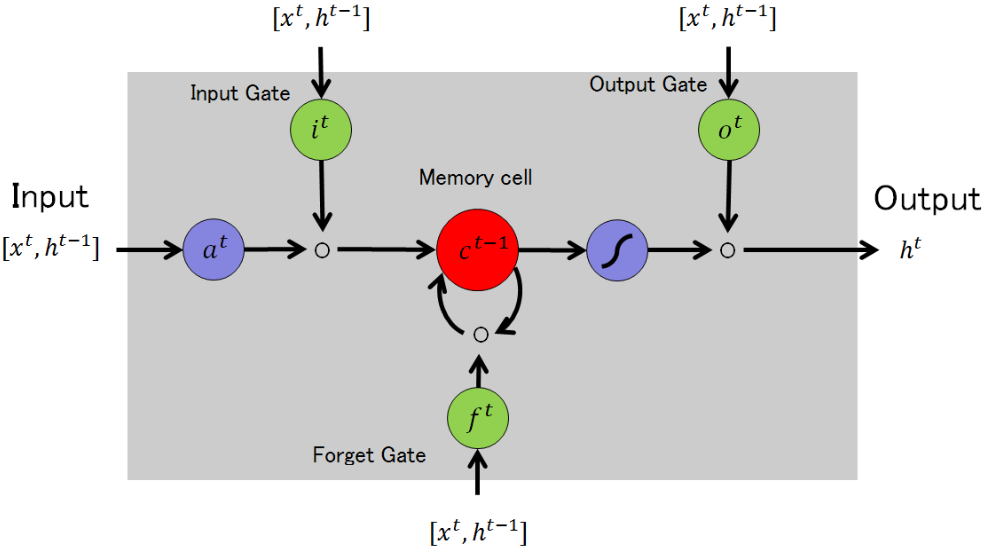
\includegraphics[width=0.7\textwidth]{gfx/rul_lstm2}
    \caption{LSTM Cell in the proposed model. \cite{DBLP:conf/icphm/ZhengRFG17} }
    \label{fig:lstm2_rul}
\end{figure}

RMSprop optimizer is used to train the model and use dropout to control overfitting. This model also aims to optimize the error function with respect to above defined variable weights and biases. The error function is given by the ,
\begin{equation}
    E = \sum_{i=1}^{t} \mid \mid y_i - \hat{y_i} \mid \mid^2
\end{equation}
Different types of sensors are used and the value scale for each of those also vary, this calls for normalization of sensor data before it is used for training or testing. Two normalizations, \textbf{z-score} normalization and \textbf{min-max} normalization are applied to the data,\\
\textbf{z-score normalization}
\begin{equation}
    x_i^\prime = \frac{x_i - \mu_i}{\sigma_i}
\end{equation}
\textbf{min-max normalization}
\begin{equation}
    x_i^\prime = \frac{x_i - min(x_i)}{max(x_i)-min(x_i)}
\end{equation}
Proposed structure is adequate for RUL estimation due to the fact that this LSTM approach \cite{DBLP:conf/icphm/ZhengRFG17} utilizes the complementarity modeling capability of LSTM and NN. LSTM is responsible for temporal modeling. NN is good at mapping LSTM feature to regression outcomes.

\section{Evaluation Setup}
\vspace*{-12.5mm}\hfill{\fontfamily{phv}\normalsize\emph{Vinay Kaundinya}}
\label{sec:rul_estimation:evaluation_setup}

To compare performance of a different models, we need to define few objective performance measures. Looking into the approaches described above, we employ the following symmetric and asymmetric functions as part of performance measures

\subsection{Symmetric Loss Functions}
\label{sec:rul_estimation:evaluation_setup:sym_loss}

\subsubsection*{RMSE}

Root Mean Squared Error(RMSE) is chosen as one of the performance measures in predicting RUL. This is a symmetric function, which penalizes both early and late predictions by giving them equal weights. We define RMSE in equation \ref{rmse:eq1},
\begin{equation} \label{rmse:eq1}
    RMSE = \sqrt{\frac{1}{N}\sum^{N}_{i=1}(y_{i} - \hat{y_{i}})^2}
\end{equation}
Here, $N$ is the total number of cycles in the time series and $y_{i} - \hat{y_{i}}$ is the difference between the predicted RUL value and the actual RUL value. We look at the RMSE values for each approach and the approach with lower RMSE value is chosen as a better approach.

\subsubsection*{MAPE}

Mean Absolute Percentage Error(MAPE) is the other chosen performance measure which is also symmetric in nature. MAPE is nothing but the mean or average of the absolute difference of predicted and actual RUL values, expressed in percentages.
\begin{equation}
    MAPE = \frac{100}{N}\sum^{N}_{i=1}\frac{\mid y_{i} - \hat{y_{i}} \mid}{\hat{y_{i}}}
\end{equation}
Here, $y_{i}$ is the predicted RUL value and $\hat{y_{i}}$ is the actual RUL value. MAPE values are percentages and hence makes it easier to compare Error percentages of different approaches. Approach with smaller MAPE is the better approach.

\subsection{Asymmetric Loss Functions}
\label{sec:rul_estimation:evaluation_setup:asym_loss}
We know that neural networks aim to minimize the errors by adjusting weights in each layer so that the correct mapping of input to output happens, during the training process. Symmetric loss functions might fall short in penalizing cases where early prediction and late prediction do not have the same effect, specially here in our case of estimating RUL for a component. Hence, we define a few asymmetric loss functions in this section, that can be used to penalize an early prediction differently from a late prediction.
\subsubsection*{LIN-LIN}
Given a test dataset and a model to predict, we can easily compute the absolute error loss by finding an absolute difference between the actual RUL $\hat{y_{i}}$ and the predicted RUL $y_{i}$ values. Absolute error loss function $f_{AE}$ defined in equation \ref{lin:eq2} is a symmetric function.
\begin{equation} . \label{lin:eq2}
    f_{AE}(\hat{y_{i}},y_{i}) = \mid \hat{y_{i}} - y_{i} \mid
\end{equation}
In order to convert this loss function into an asymmetric loss function, we then introduce weights $a$ and $b$ which will be multiplied to the loss function. Now we get a function (\ref{lin:eq1}), which incase of $a \neq b$ becomes an asymmetric loss function, known as $LIN-LIN$ asymmetric loss function.
\begin{equation} \label{lin:eq1}
    f_{LIN-LIN}(a, b,\hat{y_{i}},y_{i}) = \begin{cases}
        -a(\hat{y_{i}} - y_{i}),\hspace{1cm}if \hat{y_{i}} - y_{i} \leq 0 \\
        b(\hat{y_{i}} - y_{i}),\hspace{1cm}otherwise
    \end{cases}
\end{equation}

\subsubsection*{Score}

We define another loss function called $Score$ function ($S$) as an important objective performance measure,
\begin{equation}
    S = \begin{cases}
        \sum^{N}_{i=1}(e^{-\frac{y_i-\hat{y_i}}{13}}-1),\hspace{1cm} if y_i - \hat{y_i} < 0 \\
        \sum^{N}_{i=1}(e^{\frac{y_i-\hat{y_i}}{10}}-1),\hspace{1cm} if y_i - \hat{y_i} \geq 0
    \end{cases}
\end{equation}
Here, the late predictions or cases where its too late to perform maintenance are penalized more than the early predictions. In case of early prediction, one has enough time to perform maintenance. The lower the Score function value the better is the approach or model being tested.

\subsubsection*{Performance}

We also introduce another metric that evaluates the overall algorithm accuracy called Performance. According to this metric all prediction values must be within an acceptable range to be considered as correct prediction. The acceptable range is $[-10, 13]$. This provides a percentage of correct predictions, whereas $score$ gives us an idea of the overall error.